\section{Regional Closed-Karst Cold-Air Pooling Compresses the Growing Season}
\label{sec:regional_karst}

A single valley cannot separate general geomorphic physics from site history. Scanning the Southern Cumberland Plateau with offline Priority-Flood depression filling identified 17 closed basins ($\ge 22.5$~m sill depth, $\ge 0.30~\text{km}^2$). Six basins fell below the 60\% deciduous-floor threshold (\texttt{NLCD-41}) and were excluded prior to regional phenology extraction: \texttt{Karst\_TN\_04} (0\% deciduous, quarry/developed), \texttt{Karst\_TN\_06} (35.4\% 30~m \texttt{NLCD-41}, 58.1\% pasture), \texttt{Karst\_TN\_13} (24.2\% \texttt{NLCD-41}), \texttt{Karst\_AL\_15} (which collapsed to 0~m fill depth at 30~m resolution), \texttt{Lost\_Cove\_TN} (48.7\% 30~m \texttt{NLCD-41}, 38.4\% pasture), and \texttt{Sinking\_Cove\_TN} (57.1\% 30~m \texttt{NLCD-41}). Notably, \texttt{Lost\_Cove\_TN} and \texttt{Sinking\_Cove\_TN} therefore sit outside the 11~regional phenology pairs and later join five of those pairs in the seven-cove \texttt{ECOSTRESS} thermal tile (\cref{sec:thermal_25yr}). The remaining 11 forested closed-karst basins span 170~km from Tennessee into northern Alabama (9 meeting the strict 30~m cutoff of $\text{FillDepth} \ge 25$~m and area $\ge 0.35~\text{km}^2$) and were matched 1:1 with adjacent open-drainage gorges (\cref{tab:karst_census}).

\begin{figure}[t]
\centering
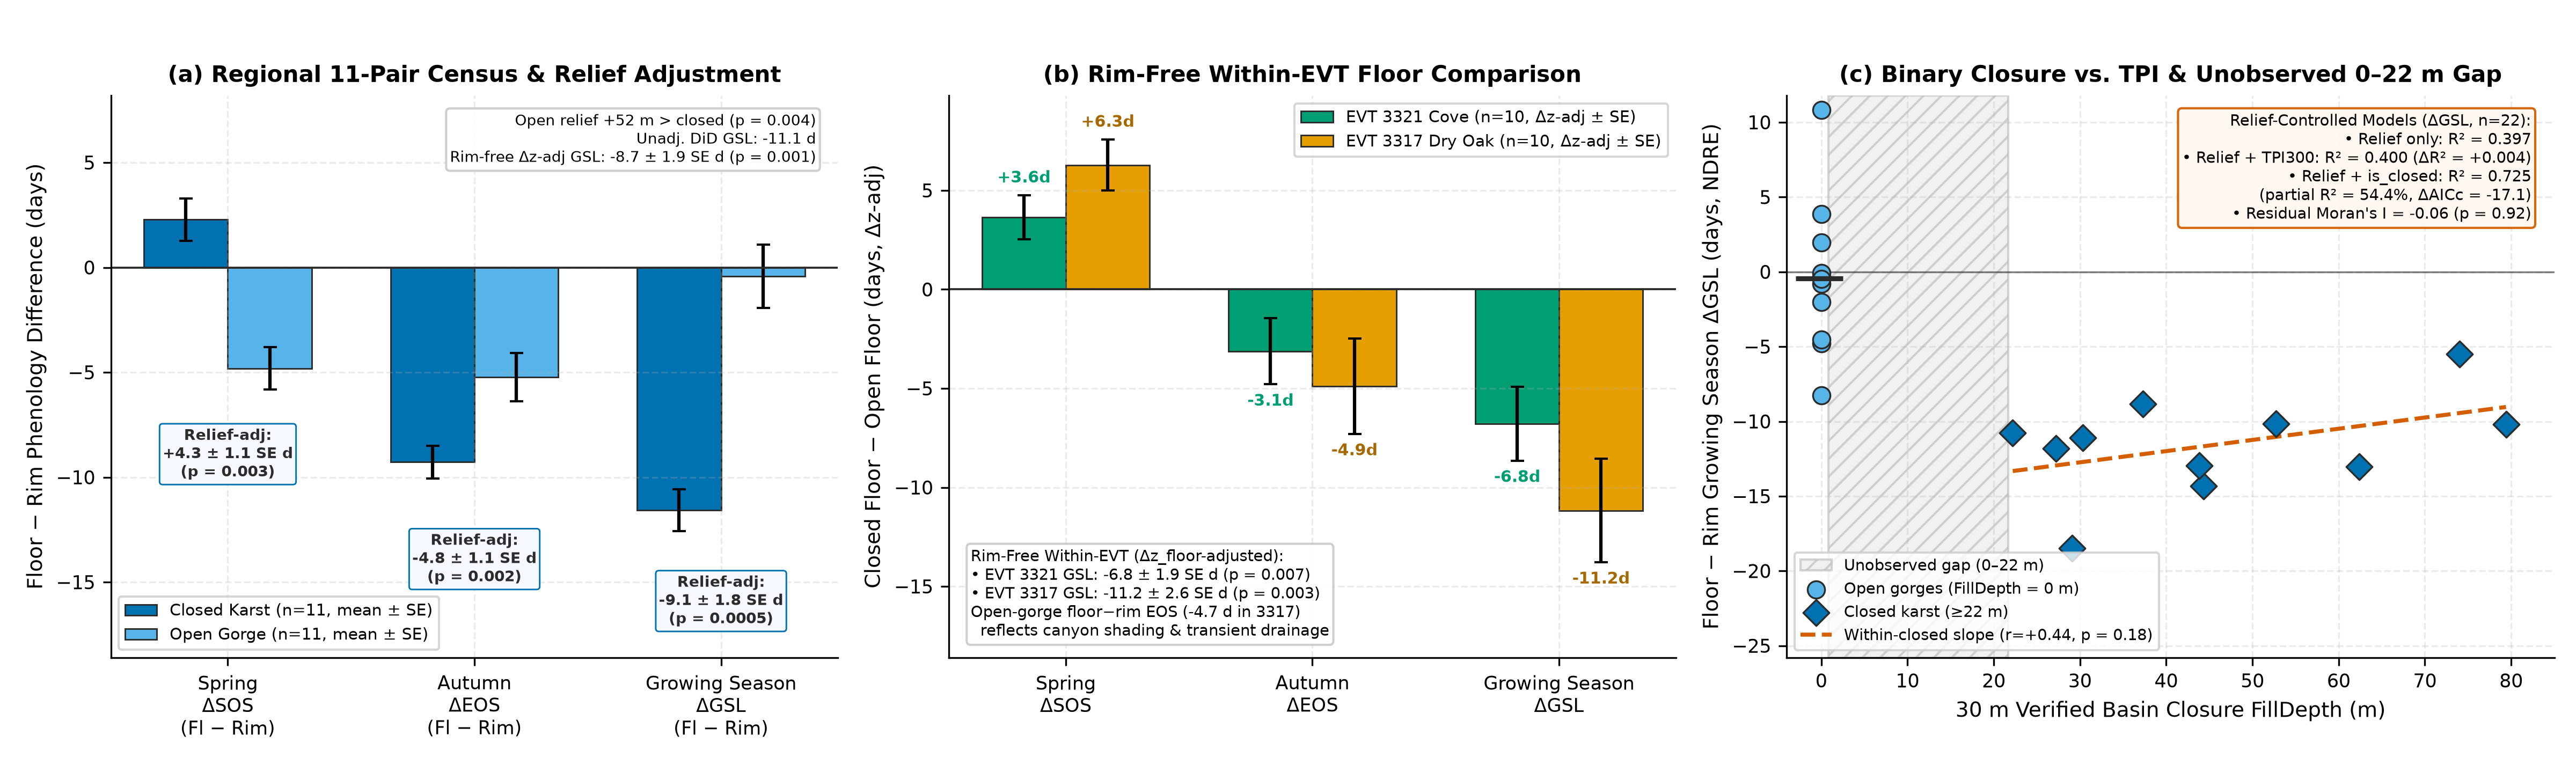
\includegraphics[width=\linewidth]{figures/fig3.png}
\caption{\textbf{Closed karst basins compress growing seasons after relief and rim-free controls.} (a)~Floor-minus-rim NDRE (mean $\pm$ SE) across 11 closed (dark blue) vs.\ 11 open basins (light blue), annotated with relief-adjusted CR1 estimates ($\Delta\text{GSL}=-9.1 \pm 1.8$~d SE, $p=0.0005$). (b)~Rim-free $\Delta z_{\text{floor}}$-adjusted differences persist within identical dry oak (\texttt{EVT 3317}, $-11.2$~d) and cove (\texttt{EVT 3321}, $-6.8$~d) classes. (c)~Binary closure adds 54.4\% partial $R^2$ over relief ($\Delta\text{AIC}_c=-17.1$ vs.\ TPI), with 0--22~m sills unobserved (hatched) and no ramp above 22~m.}
\label{fig:regional_karst}
\end{figure}

\subsection{Relief-Adjusted Inference and Rim-Free Floor-vs-Floor Verification}
Auditing pair geometry revealed a systematic relief imbalance: open-drainage controls have 51.8~m greater floor-to-rim relief than closed basins (mean $178.3 \pm 53.6$~m SD vs.\ $126.5 \pm 41.2$~m SD, paired $p=0.0043$), and 7/11 open rims sit at or above 535~m elevation (where the plateau-cap spring lag operates) compared with 2/11 closed rims. Greater elevation relief alone shifts open floor-minus-rim $\Delta\text{SOS}$ more negative and inflates the unadjusted paired Difference-in-Differences (NDRE unadjusted DiD: $\Delta\text{SOS}=+7.09$~d, $\Delta\text{EOS}=-4.05$~d, $\Delta\text{GSL}=-11.14$~d; NDVI unadjusted $\Delta\text{GSL}=-10.67$~d).

Adjusting 22-site NDRE regressions explicitly for floor-to-rim relief with CR1 pair-clustered standard errors ($\text{df}=10$) confirms a smaller but well-supported growing-season compression (\cref{fig:regional_karst}a, \cref{tab:karst_census}): closed basins delay spring by $+4.28 \pm 1.13$~d (SE, $p=0.0035$), advance autumn by $-4.79 \pm 1.13$~d (SE, $p=0.0017$), and shorten the growing season by $-9.07 \pm 1.81$~d (SE, $p=0.00053$), with no $\text{is\_closed} \times \text{relief}$ interaction ($p=0.66$--$0.86$). NDVI yields a consistent relief-adjusted compression ($\Delta\text{SOS}=+4.20 \pm 1.21$~d SE, $p=0.0059$; $\Delta\text{EOS}=-3.84 \pm 1.26$~d SE, $p=0.012$; $\Delta\text{GSL}=-8.04 \pm 2.10$~d SE, $p=0.0034$), and the strict 30~m nine-pair subset behaves similarly ($\Delta\text{GSL}=-10.20 \pm 2.04$~d SE in NDRE, $p=0.0011$).

To bypass rim elevation and plateau-cap effects altogether, we also compared closed and open \emph{floors} directly while adjusting for residual floor-elevation differences ($\Delta z_{\text{floor}}$, mean $+12.3$~m). Across all 11 pairs in NDRE, rim-free $\Delta z_{\text{floor}}$-adjusted floor-vs-floor regression yields $\Delta\text{SOS}=+5.56 \pm 1.15$~d (SE, $p=0.00095$), $\Delta\text{EOS}=-3.19 \pm 1.38$~d (SE, $p=0.047$), and $\Delta\text{GSL}=-8.75 \pm 1.85$~d (SE, $p=0.0011$). Stratifying floors strictly within identical \texttt{LANDFIRE} ecological types ($n=10$ valid pairs per class, $\Delta z_{\text{floor}}$-adjusted) shows that growing-season compression persists inside both \texttt{EVT 3317} dry oak forest ($\Delta\text{SOS}=+6.28 \pm 1.29$~d SE, $p=0.0012$; $\Delta\text{EOS}=-4.89 \pm 2.41$~d SE, $p=0.077$; $\Delta\text{GSL}=-11.17 \pm 2.61$~d SE, $p=0.0027$) and \texttt{EVT 3321} mesophytic cove forest ($\Delta\text{SOS}=+3.65 \pm 1.10$~d SE, $p=0.011$; $\Delta\text{EOS}=-3.13 \pm 1.67$~d SE, $p=0.098$; $\Delta\text{GSL}=-6.78 \pm 1.87$~d SE, $p=0.0067$; \cref{fig:regional_karst}b). Closed floors contain more dry oak (57.7\% \texttt{EVT 3317}) and less cove forest (25.6\% \texttt{EVT 3321}) than open floors (44.0\% \texttt{EVT 3321}), ruling out mesophytic species enrichment as the cause.

Under internal decision criterion P1, we record the overall status transparently as \texttt{PARTIAL\_PASS}: although every closed basin (11/11) senesces earlier on its floor than its rim ($-9.28 \pm 2.57$~d SD in NDRE) and paired/relief-adjusted tests pass, two sub-criteria failed: open-gorge controls themselves showed $-3.03$~d (NDVI) to $-5.23$~d (NDRE) floor-minus-rim EOS (reflecting canyon shading and transient drainage even within identical \texttt{EVT 3317}, $-4.74$~d, $p=0.0048$), and $r(\sigma_{\text{SOS}}, \text{FillDepth})$ reached 0.22 in NDVI (exceeding the 0.15 internal threshold).

\begin{table}[t]
\centering
\begin{threeparttable}
\caption{\textbf{Regional closed-karst phenology (NDRE, $N=11$ pairs) and relief-controlled geomorphic models.} All $\pm$ values denote SE (CR1 pair-clustered $\text{df}=10$ in Part~A OLS; OLS $\text{df}=n-2$ in rim-free comparisons).}
\label{tab:karst_census}
\footnotesize
\setlength{\tabcolsep}{4.0pt}
\begin{tabularx}{\linewidth}{@{} >{\raggedright\arraybackslash}X c r r r @{}}
\toprule
Estimator / Model & $n$ & Spring $\Delta$SOS (d) & Autumn $\Delta$EOS (d) & $\Delta$GSL (d) \\
\midrule
\multicolumn{5}{@{}l}{\textit{Part A: Closed-Karst vs.\ Open-Gorge Effects (NDRE)}} \\
\textbf{Relief-adj.\ 22-site CR1 OLS (primary)} & 11 pairs & $+4.28 \pm 1.13$ ($0.0035$) & $-4.79 \pm 1.13$ ($0.0017$) & $\mathbf{-9.07 \pm 1.81}$ ($0.0005$) \\
Relief-adj.\ 22-site CR1 OLS (NDVI) & 11 pairs & $+4.20 \pm 1.21$ ($0.0059$) & $-3.84 \pm 1.26$ ($0.012$) & $-8.04 \pm 2.10$ ($0.0034$) \\
Rim-free floor-vs-floor ($\Delta z_{\text{fl}}$-adj.) & 11 pairs & $+5.56 \pm 1.15$ ($0.0010$) & $-3.19 \pm 1.38$ ($0.047$) & $-8.75 \pm 1.85$ ($0.0011$) \\
Within \texttt{EVT 3317} dry oak ($\Delta z_{\text{fl}}$-adj.) & 10 pairs & $+6.28 \pm 1.29$ ($0.0012$) & $-4.89 \pm 2.41$ ($0.077$) & $-11.17 \pm 2.61$ ($0.0027$) \\
Within \texttt{EVT 3321} cove ($\Delta z_{\text{fl}}$-adj.) & 10 pairs & $+3.65 \pm 1.10$ ($0.011$) & $-3.13 \pm 1.67$ ($0.098$) & $-6.78 \pm 1.87$ ($0.0067$) \\
Unadjusted paired DiD (for reference) & 11 pairs & $+7.09 \pm 1.23$ ($0.0002$) & $-4.05 \pm 1.08$ ($0.0038$) & $-11.14 \pm 1.63$ ($4.4{\times}10^{-5}$) \\
\midrule
\multicolumn{5}{@{}l}{\textit{Part B: Relief-Controlled Geomorphic Models Across 22 Sites ($R^2$ and $\text{AIC}_c$ on NDRE $\Delta$GSL)}} \\
Relief only & 22 & \multicolumn{3}{r}{$R^2=0.397$, $\text{AIC}_c=143.5$ ($\Delta\text{AIC}_c=+14.3$ vs.\ best)} \\
Relief + 300~m TPI & 22 & \multicolumn{3}{r}{$R^2=0.400$ ($\Delta R^2=+0.004$), $\text{AIC}_c=146.4$ ($\Delta\text{AIC}_c=+17.1$)} \\
Relief + linear \texttt{FillDepth} & 22 & \multicolumn{3}{r}{$R^2=0.580$, $\text{AIC}_c=138.6$ ($\Delta\text{AIC}_c=+9.3$)} \\
\textbf{Relief + binary \texttt{is\_closed}} & 22 & \multicolumn{3}{r}{$\mathbf{R^2=0.725}$ (partial $R^2=54.4\%$), $\mathbf{\text{AIC}_c=129.3}$ ($\Delta\text{AIC}_c=0.0$)} \\
\bottomrule
\end{tabularx}
\begin{tablenotes}[flushleft]
\footnotesize
\item Parentheses in Part~A give two-sided $p$-values. Internal gate P1 status: \texttt{PARTIAL\_PASS}.
\end{tablenotes}
\end{threeparttable}
\end{table}

\subsection{Binary Topographic Closure vs.\ Local Concavity (0--22~m Unobserved)}
Open gorges and closed karst valleys share nearly identical local concavity (mean 300~m TPI of $-11.5$~m vs.\ $-13.4$~m), so adding 300~m TPI to relief explains virtually no additional variance in NDRE $\Delta\text{GSL}$ ($R^2=0.397$ to $0.400$, $\Delta R^2=+0.004$; \cref{tab:karst_census}). Adding binary topographic closure (\texttt{is\_closed}) lifts $R^2$ from $0.397$ to $0.725$ (partial $R^2=54.4\%$ over relief; $\Delta\text{AIC}_c=-17.1$ relative to relief plus 300~m TPI and $-14.3$ relative to relief alone), with negligible spatial autocorrelation in residuals (permutation Moran's $I=-0.06, p=0.92$).

Importantly, this is a binary closure contrast rather than a continuous depth-response curve (\cref{fig:regional_karst}c). Because all 11 open gorges have $\text{FillDepth}=0$~m and all 11 closed basins have 30~m $\text{FillDepth}$ between 22.2 and 79.4~m, a 25~m saturating hinge equals $25 \times \text{is\_closed}$ on 21/22 sites ($\Delta\text{AIC}_c=0.03$). Within the 11 closed basins above 22~m, deeper 30~m sills do not intensify compression ($r(\Delta\text{EOS}, \text{FillDepth})=+0.26, p=0.45$; $r(\Delta\text{GSL}, \text{FillDepth})=+0.44, p=0.18$), and the shallow 0--22~m sill regime remains unobserved in this regional sample.
